\documentclass[a4paper,10pt]{article}
\usepackage[utf8]{inputenc}
\usepackage[english]{babel}
\usepackage{geometry}
\usepackage[T1]{fontenc}
\usepackage{float}
\usepackage{multirow}
\usepackage{booktabs}
\usepackage{chemfig}
\usepackage{amsmath}
\usepackage{xcolor}
\usepackage{pxfonts}
\usepackage{tikz}
\usepackage{listings}

\definecolor{dkgreen}{rgb}{0,0.6,0}
\definecolor{gray}{rgb}{0.5,0.5,0.5}
\definecolor{mauve}{rgb}{0.58,0,0.82}

\title{Xtext Tutorial}
\author{}



\newcommand{\gerquot}[1]{\glqq#1\grqq}
\newcommand{\dashAndSpace}{\textendash \space}
\newcommand{\dashAndSpaceSeq}[1]{\dashAndSpace#1 \textendash}
\newcommand{\leadingFourCharTab}{\phantom{XXXX}}

\newcommand{\DSL}{domain specific language}
\newcommand{\CFG}{context-free grammar}
\newcommand{\IUPAC}{International Union of Pure and Applied Chemistry}
\newcommand{\EMF}{Eclipse Modeling Framework}
\newcommand{\EBNF}{Extended Backus-Naur Form}

\newcommand{\captionVSpace}{\vspace*{-0.05cm}}
\newcommand{\screenshotWidth}{0.975}

\newcommand{\colorChain}{red}
\newcommand{\colorChainName}{\colorChain\space}
\newcommand{\colorBranchOne}{green}
\newcommand{\colorBranchOneName}{\colorBranchOne\space}
\newcommand{\colorBranchTwo}{orange}
\newcommand{\colorBranchTwoName}{\colorBranchTwo\space}

\newcommand{\IUPACExample}[1]{\texttt{#1}\\}


%%%%% %%%%% %%%%% %%%%% %%%%% %%%%% %%%%% %%%%%                %%%%% %%%%% %%%%% %%%%% %%%%% %%%%% %%%%% %%%%%
%%%%% %%%%% %%%%% %%%%% %%%%% %%%%% %%%%% %%%%% BEGIN document %%%%% %%%%% %%%%% %%%%% %%%%% %%%%% %%%%% %%%%%
%%%%% %%%%% %%%%% %%%%% %%%%% %%%%% %%%%% %%%%%                %%%%% %%%%% %%%%% %%%%% %%%%% %%%%% %%%%% %%%%%
\begin{document}

\maketitle

\section{Syntax Overview}
In this chapter we show a syntax overview of Xtext with a meta model of a real-world example. Instead of using the generated Xtext code, we will rewrite the default grammar, generated by Xtext, into a simpler, more human-friendly one. A hands-on guide for using Xtext in Eclipse, with instructions on how to exactly generate the infrastructure and to run the generated editor is given in Chapter AD.

The Xtext specification language is a variation of the familiar \EBNF\space(EBNF) notation for context free grammars. EBNF is used by most parser generators, and it is included in curriculum of most compiler courses.

We shall now discuss the main syntactic elements of the Xtext language, by presenting a simple grammar based on a tiny subset of the IUPAC nomenclature, whose meta-model is shown in Fig. \ref{fig:SSIUPACMetaModel}.

\gerquot{IUPAC} is the abbreviation for \gerquot{\IUPAC} and is a nomenclature system, that is widely used in the chemistry. Main goal of this naming system is the encoding of chemical structures in a text-based name.

The two main components are chains and branches of carbon atoms. One part of the molecule is defined as chain and the rest are the branches. Every branch has the information on which carbon atom on the chain is connected to. The length information is simply substituted with a name. See table \ref{tab:NumCarbonChainEncodedName} for the substitution of chains and table \ref{tab:NumCarbonBranchEncodedName}.

%%%%% BEGIN Table with the substitutions of a chain %%%%%
\begin{table}[H]
    \centering
    \begin{tabular}{c|l}
        \toprule
        \textbf{Number of carbon atoms in branch} & \textbf{Encoded name} \\
        \midrule
        1 & Methan \\
        2 & Ethan \\
        3 & Propan \\
        4 & Butan \\
        5 & Pentan \\
        6 & Hexan \\
        7 & Heptan \\
        8 & Octan \\
        9 & Nonan \\
        10 & Decan \\
        \bottomrule
    \end{tabular}
    \captionVSpace
    \caption{List of the first 10 names for a chain}
    \label{tab:NumCarbonChainEncodedName}
\end{table}
%%%%% END Table with the substitutions of a chain %%%%%

For the encoded branch names the postfix \gerquot{an} of the encoded chain names is replaced with \gerquot{yl}.

%%%%% BEGIN Table with the substitutions of a branch %%%%%
\begin{table}[H]
    \centering
    \begin{tabular}{c|l}
        \toprule
        \textbf{Number of carbon atoms in branch} & \textbf{Encoded name} \\
        \midrule
        1 & Methyl \\
        2 & Ethyl \\
        3 & Propyl \\
        4 & Butyl \\
        \bottomrule
    \end{tabular}
    \captionVSpace
    \caption{List of the first 4 names for a branch}
    \label{tab:NumCarbonBranchEncodedName}
\end{table}
%%%%% END Table with the substitutions of a chain %%%%%

Usually if a branch with the same length occurs multiple times, these branches are summarized in one branch term and the number of branches with this length is also substituted with a string. The table \ref{tab:BranchesWithTheSameLength} shows the first four elements. We call this element \gerquot{summary prefix}.

%%%%% BEGIN Table with the substitutions of multiple branches with the same length %%%%%
\begin{table}[H]
    \centering
    \begin{tabular}{c|l}
        \toprule
        \textbf{Branches with the same length} & \textbf{Prefix} \\
        \midrule
        1 & Mono \\
        2 & Di \\
        3 & Tri \\
        4 & Tetra \\
        \bottomrule
    \end{tabular}
    \captionVSpace
    \caption{List of the first 4 prefixes to summarize branches with the same length}
    \label{tab:BranchesWithTheSameLength}
\end{table}
%%%%% END Table with the substitutions of multiple branches with the same length %%%%%

In the following example the chain is \colorChainName and the branch are drawn \colorBranchOneName.

%%%%% BEGIN First IUPAC example %%%%%
\begin{figure}[H]
\noindent\IUPACExample
{
    \color{\colorChain}{C - C - C - C}\\
    \phantom{XXXXX}\color{\colorBranchOne}{|}\\
    \phantom{XXXXX}\color{\colorBranchOne}{C}
}
\caption{Chain length 4 $\rightarrow$ \gerquot{Butan}; One branch with length 1 $\rightarrow$ \gerquot{MonoMethyl}; Position of the branch: 2\space\space\space Result: \textbf{2-MonoMethylButan}}
\end{figure}
%%%%% END First IUPAC example %%%%%

The order of the components is: Position(s) + minus sign + summary prefix + encoded branch length + encoded chain length. In the case, that there is no branch, only the encoded chain length literal will be used. The next example shows, that this order is also valid for multiple different branches.

%%%%% BEGIN Second IUPAC example %%%%%
\begin{figure}[H]
\noindent\IUPACExample
{
    \color{\colorChain}{C - C - C - C - C - C - C}\\
    \phantom{XXXXXXXXXXXXX}\color{\colorBranchTwo}{|}\phantom{XXX}\color{\colorBranchOne}{|}\phantom{XXX}\color{\colorBranchOne}{|}\\
    \phantom{XXXXXXXXXXXXX}\color{\colorBranchTwo}{C}\phantom{XXX}\color{\colorBranchOne}{C}\phantom{XXX}\color{\colorBranchOne}{C}\\
    \phantom{XXXXXXXXXXXXX}\color{\colorBranchTwo}{|}\\
    \phantom{XXXXXXXXXXXXX}\color{\colorBranchTwo}{C}
}
\caption{Chain length 7 $\rightarrow$ \gerquot{Heptan}; Two branches with length 1 on position 2 and 3 $\rightarrow$ \gerquot{2,3-DiMethyl}; One branch with length 2 on position 4 $\rightarrow$ \gerquot{4-MonoEthyl}\space\space\space Result: \textbf{2-MonoEthyl-3,4DiMethylButan}}
\end{figure}
%%%%% END Second IUPAC example %%%%%

Figure \ref{fig:SSIUPACMetaModel} shows a possible abstract syntax (the meta model) of the IUPAC nomenclature.

%%%%% BEGIN Meta Model Screenshot %%%%%
\begin{figure}[H]
\centering
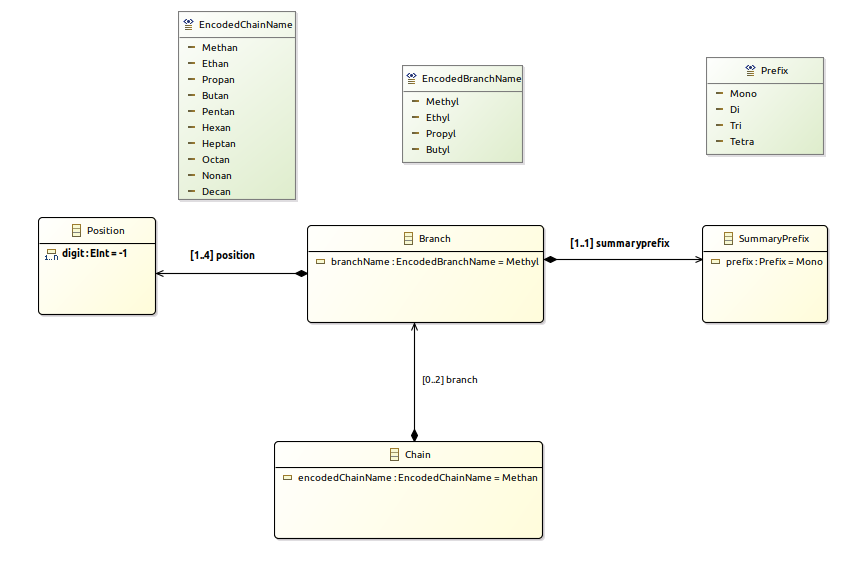
\includegraphics[width=\screenshotWidth\textwidth]{./Screenshots/Overview.png}
\caption{Meta model of the IUPAC nomenclature.}
\label{fig:SSIUPACMetaModel}
\end{figure}
%%%%% END Meta Model Screenshot %%%%%

Terminals are simply introduced as string literals. Enums are in this context also kind of terminals. For the enum \emph{Prefix}, the code look like:\\

\noindent\texttt{enum Prefix returns Prefix:\\
\leadingFourCharTab\leadingFourCharTab Mono = 'Mono' | Di = 'Di' | Tri = 'Tri' | Tetra = 'Tetra';}\\

Here is important to notice, that the element left from the equal char is one of the enum entries and on the right side is the coressponding string literal. This double usage in Xtext sounds unnecessary, but the reason for this syntax descision is, that an enum entry could also have coressponding literals, that are different from the enum entry name.

Nonterminal symbols uses the property name, that was defined in the meta model. In addition the type of the property will be included here. The nonterminal \gerquot{Position} could have the following implementation:\\

\noindent\texttt{Position returns Position:\\
\leadingFourCharTab\leadingFourCharTab digit=EInt ("," digit+=EInt)*;}\\

We see here also the grouping operator and the repetition-symbol from EBNF. The \texttt{+=} operator adds content to a property instead of assigning. A value resulting from parsing a nonterminal can be stored directly in a property of the current abstract syntax object. The meaning of the complete nonterminal: \emph{A digit plus unlimited optional digits, that needs to be started with a comma char.}\\

Due to the composition relations between the classes, the class \gerquot{Chain} is the class higest order and contains all other classes with direct oder indirect relations. We see in the description of the IUPAC nomenclature, that only a instance of the Chain class is mandatory. In Xtext such a mandatory can be expressed with braced char:\\

\noindent\texttt{Chain returns Chain:\\
\leadingFourCharTab\{Chain\}\\
\leadingFourCharTab\leadingFourCharTab(branch+=Branch (branch+=Branch)*)?\\
\leadingFourCharTab\leadingFourCharTab(encodedChainName=EncodedChainName);}\\

Don't be confused with the repetition meaning in EBNF! In Xtext a repetition can only be written with the char \emph{*} and \emph{+}. The question mark has the same meaning compared to EBNF; it describes that an terminal or nonterminal is optional.\\

Vergleichstabelle Xtext EBNF\\
Kompletten Xtext Code hier anzeigen.\\

There is much more to Xtext than we present, but this is sufficient for creating simple languages. Among other elements, of the highest interest are probably customizable scoping semantics (what names are visible in what scopes), and fully qualified name support for references across name spaces/scopes. These are described in the Xtext documentation.

Finally, C-like comments (both block comments, and line comments) are automatically supported in languages built with Xtext.


\end{document}
%%%%% %%%%% %%%%% %%%%% %%%%% %%%%% %%%%% %%%%%              %%%%% %%%%% %%%%% %%%%% %%%%% %%%%% %%%%% %%%%%
%%%%% %%%%% %%%%% %%%%% %%%%% %%%%% %%%%% %%%%% END document %%%%% %%%%% %%%%% %%%%% %%%%% %%%%% %%%%% %%%%%
%%%%% %%%%% %%%%% %%%%% %%%%% %%%%% %%%%% %%%%%              %%%%% %%%%% %%%%% %%%%% %%%%% %%%%% %%%%% %%%%%
